%% LyX 1.5.3 created this file.  For more info, see http://www.lyx.org/.
%% Do not edit unless you really know what you are doing.
\documentclass[english]{llncs}
\usepackage[T1]{fontenc}
\usepackage[latin9]{inputenc}

\makeatletter

%%%%%%%%%%%%%%%%%%%%%%%%%%%%%% LyX specific LaTeX commands.
%% Bold symbol macro for standard LaTeX users
\providecommand{\boldsymbol}[1]{\mbox{\boldmath $#1$}}


%%%%%%%%%%%%%%%%%%%%%%%%%%%%%% User specified LaTeX commands.
\usepackage{ae}

\usepackage{tikz}
\usetikzlibrary{snakes}
\usetikzlibrary{arrows}
\usetikzlibrary{shapes}

\usepackage{babel}
\makeatother

\begin{document}

\title{Reasoning with Powerdomains in Isabelle/HOLCF}


\author{Brian Huffman}


\institute{Portland State University\\
\email{brianh@cs.pdx.edu}}

\maketitle
\begin{abstract}
This paper presents the first fully-mechanized formalization of powerdomains,
implemented in the HOLCF logic of the Isabelle theorem prover. The
powerdomain library provides an abstract view of powerdomains to the
user, hiding the complicated implementation details. The library also
provides proof automation, in the form of sets of rewrite rules for
solving equalities and inequalities on powerdomains.
\end{abstract}

\section{Introduction}

Powerdomains are a domain-theoretic analog of powersets, which were
designed for reasoning about the semantics of nondeterministic programs.\cite{plotkin76powerdomain}
The use of powerdomains for reasoning about nondeterminism (and domain-theoretic
denotational semantics in general) has declined in recent years, which
I believe is primarily due to their perceived complexity. Compared
to other more syntactic approaches to semantics, domain theory and
powerdomains require a lot of mathematical sophistication to understand.
This is a significant barrier for anyone who might want to use denotational
semantics to reason about computation. It is my hope that the existence
of good formalized libraries will remove that barrier to the use of
domain theory for denotational semantics.

In this paper I attempt to demonstrate that powerdomains are a natural
way for functional programmers to reason about nondeterministic programs.
Using Haskell-style monadic code as a starting point, Section \ref{sec:Nondeterminism-Monads}
motivates the definition of a powerdomain. Section \ref{sec:Powerdomains}
examines the three main varieties of powerdomains, and attempts to
convey some intuitions about their structures and what each is good
for. For readers wishing to use the powerdomain library, Section \ref{sec:HOLCF-powerdomain-library}
documents all of the powerdomain operations provided by the library,
as well as some of the lemmas and proof automation that is available.
Section \ref{sec:Implementation} describes the implementation of
the powerdomain library; understanding this section is not necessary
in order to use the library, and may be skipped on first reading.

This paper assumes some familiarity with the Haskell language. In
particular, I expect the reader to know about monads, and the monad
laws. I also assume that the reader is familiar with some of the basics
of domain theory, which is traditionally used for reasoning denotationally
about Haskell programs.\cite{bird98introduction} In particular, the
reader should know about bottoms ($\bot$), complete partial orders
($\sqsubseteq$), limits of chains, continuous functions, and admissible
predicates.


\section{\label{sec:Nondeterminism-Monads}Nondeterminism monads}

From a functional programmer's perspective, a powerdomain can be thought
of as simply a special kind of monad for nondeterminism. In addition
to the standard monad operations \emph{return} and \emph{bind}, a
powerdomain also provides a binary operation for making a nondeterministic
choice. In Haskell syntax, we can specify a subclass of monads that
have such a binary choice operator:\cite{papaspyrou00study}

\begin{verbatim}
class (Monad m) => MultiMonad m where
  (+|+) :: m a -> m a -> m a
\end{verbatim}

Haskell programmers often use the list monad to model nondeterministic
computations; functions indicate multiple possible return values by
enumerating them in a list. In this case, the list append operator
$(+\!+)$ fills the role of nondeterministic choice.

\begin{verbatim}
instance MultiMonad [] where
  xs +|+ ys = xs ++ ys
\end{verbatim}

The list monad has the great advantage of being executable: If you
code up a nondeterministic algorithm in the list monad, you can just
run it and see the results. However, for \emph{reasoning} about nondeterministic
algorithms, the list monad falls short in two important ways.

First, the list monad is not abstract enough: There are many different
lists that represent the same set of possible return values. For example,
consider a nondeterministic integer computation $f$ with three possible
outcomes: a return value of 3, a return value of 5, or divergence
(i.e. a return value of $\bot$). The lists $[3,5,\bot]$ and $[5,5,3,\bot,3]$
both represent the value of $f$ equally well; both represent the
set $\{3,5,\bot\}$. If divergence were not a possibility, then we
could canonicalize the lists by sorting and removing duplicates---but
obviously this does not work in general.

The second problem is that the list monad does not behave well in
the presence of infinite or partial output. The problem originates
with the definition of append: If $xs$ is an infinite list, then
$xs+\!\!+ys$ does not depend on $ys$ at all. If $ys$ includes some
possible outcomes that do not already occur in $xs$, then they get
thrown away. Similarly, if $xs$ is a partial list, like $1:2:\bot$,
then $xs+\!\!+ys$ also ignores its second argument.

This problem is demonstrated by the following recursive nondeterministic
computation. Any integer greater than or equal to 2 should be a possible
result. However, when interpreted in the list monad, only even integers
are included. The problem is that since the denotation of $f$ is
an infinite list, the {}``return 1'' is never reached.

\begin{verbatim}
f :: (MultiMonad m) => m Int
f = do x <- return 0 +|+ f +|+ return 1
       return (x+2)
\end{verbatim}

Another possible nondeterminism monad for Haskell is the binary tree,
whose definition is shown below. The binary tree monad solves the
second problem that lists had: Unlike the list append operator, the
\emph{Node} constructor never ignores either of its arguments, even
if the other is partial or infinite. However, the problem of multiple
representations remains; in fact this problem is even worse than before.
Since the choice operator for trees is a data constructor, it doesn't
satisfy any non-trivial equalities, while list append is at least
associative.

\begin{verbatim}
data Tree a = Leaf a | Node (Tree a) (Tree a)
 
instance Monad Tree where
  return x = Leaf x
  Leaf x >>= f = f x
  Node l r >>= f = Node (l >>= f) (r >>= f)
 
instance MultiMonad Tree where
  l +|+ r = Node l r
\end{verbatim}

For doing formal reasoning about nondeterministic computations, an
ideal nondeterminism monad should satisfy all the axioms listed in
Fig. \ref{fig:pd-laws}. We will call a monad that satisfies all seven
laws a \emph{powerdomain}. Laws 1--3 are just the standard Haskell
monad laws. Law 4 says that bind distributes over the choice operator,
and laws 5--7 state that choice is associative, commutative and idempotent.
The list monad satisfies laws 1--5, but not 6 or 7; the binary tree
monad satisfies only 1--4. There is no obvious way to define a true
powerdomain directly in Haskell, but in the next section we will see
how to define powerdomains mathematically.

%
\begin{figure}
\begin{enumerate}
\item \texttt{return x >$\!$>= f = f x}
\item \texttt{xs >$\!$>= return = xs}
\item \texttt{(xs >$\!$>= f) >$\!$>= g = xs >$\!$>= (\textbackslash{}x
-> f x >$\!$>= g)}
\item \texttt{(xs +|+ ys) >$\!$>= f = (xs >$\!$>= f) +|+ (ys >$\!$>=
f)}
\item \texttt{(xs +|+ ys) +|+ zs = xs +|+ (ys +|+ zs)}
\item \texttt{xs +|+ ys = ys +|+ xs}
\item \texttt{xs +|+ xs = xs}
\end{enumerate}
\caption{\label{fig:pd-laws}The powerdomain laws}

\end{figure}


Note that in addition to the seven powerdomain laws, there is another
implicit requirement for powerdomains: All of the operations must
be monotone and continuous, i.e. they must respect the cpo structure
of the types on which they operate. In Haskell, every definable function
is automatically continuous by construction, while in Isabelle, the
logic permits the definition of functions which are not necessarily
continuous. Continuity is a concept defined in Isabelle/HOLCF, and
it is necessary to prove that each function defined in the library
is continuous.


\section{\label{sec:Powerdomains}Powerdomains}

There are multiple ways to define a powerdomain with operations that
satisfy all of the desired laws. The three most common are known as
the upper, lower, and convex powerdomains. These are also respectively
known as the Smyth, Hoare, and Plotkin powerdomains. Historically,
each variety is also associated with a musical symbol: sharp ($\sharp$)
for upper, flat ($\flat$) for lower, and natural ($\natural$) for
the convex powerdomain.

Before we dive into the details of the various powerdomains, first
let us introduce some more notation. We will borrow the variable naming
convention often used for lists in Haskell: For values of powerdomain
types we use names like $xs$, $ys$, or $zs$, while for the underlying
elements we use names like $x$, $y$, or $z$.

Also, we will consistently use set-style notation when talking about
powerdomains. The singleton set syntax $\{-\}$ denotes the monadic
return operator, {}``unit''; and the set union symbol $(\cup)$
denotes the nondeterministic choice operator, {}``plus''. Also,
we will use set enumerations like $\{x,y,z\}$ as shorthand for $\{x\}\cup\{y\}\cup\{z\}$.
When necessary, we will indicate a specific powerdomain by using the
appropriate musical symbol as a superscript.


\subsection{Convex powerdomain}

For a given element domain $\alpha$, the convex powerdomain $\mathcal{P}^{\natural}(\alpha)$
is the \emph{free continuous domain-algebra} over the constructors
$\{-\}^{\natural}$ and $(\cup^{\natural})$, modulo the associativity,
commutativity, and idempotence of $(\cup^{\natural})$. (This construction
is explained in \cite[\S6.1]{abramsky94domain}) The convex powerdomain
is {}``universal'' in a category-theoretical sense, in that there
is a unique mapping (preserving unit and plus) from the convex powerdomain
into any other powerdomain.

Freeness means two things here. First, it says that the convex powerdomain
consists only of values that can be built up from applications of
unit and plus (i.e. the convex powerdomain has {}``no junk''). Secondly,
freeness also means that no nontrivial equalities between terms should
hold, except those required by the laws (i.e. the convex powerdomain
has {}``no confusion'').

In the context of complete partial orders, the {}``no junk'' property
has a slightly different meaning than it does for ordinary inductive
datatypes. As a cpo, the convex powerdomain includes values built
from a finite number of constructor applications, plus additional
values that result as limits of chains. Thus the convex powerdomain
has an induction rule like the following: \begin{equation}
\begin{array}{c}
\mbox{adm}(P)\quad\forall x.\, P(\{x\}^{\natural})\quad\forall xs\, ys.\, P(xs)\longrightarrow P(ys)\longrightarrow P(xs\cup^{\natural}ys)\\
\hline \forall xs.\, P(xs)\end{array}\label{eq:pd-induct}\end{equation}
Admissibility of $P$ means that for any chain of elements $x_{i}$
such that $P(x_{i})$ holds for all $i$, $P$ must also hold for
the limit $\bigsqcup_{i}x_{i}$. This side condition reflects the
fact that some values are only expressible as limits of chains---most
induction rules in HOLCF have a similar admissibility side condition.
(HOLCF can automatically prove admissibility for most inductive predicates
used in practice.)

We still need to check that we can satisfy all of the powerdomain
laws from Fig. \ref{fig:pd-laws}. Laws 5--7 hold by construction.
We can use laws 1 and 4 as defining equations for the bind operator.
Finally, it is straightforward to prove laws 2 and 3 by induction.

\begin{definition}
We say that $x$ is a \emph{member} of $xs$ if $\{x\}\cup xs=xs$.
\end{definition}
If $xs$ represents a nondeterministic computation, and $x$ is one
of the possible results, then $x$ must be a member of $xs$. However,
the set of members is not necessarily equal to the set of possible
results. Not every conceivable set of results can be precisely represented
in the convex powerdomain, as the following theorem implies.

\begin{theorem}
\label{thm:mem-convex}Let $xs$ be a value in a convex powerdomain.
Then the set of members of $xs$ is convex-closed.
\end{theorem}
\begin{proof}
Let $x$ and $z$ be members of $xs$, and let $y$ be any value between
$x$ and $z$, such that $x\sqsubseteq y$ and $y\sqsubseteq z$.
We will show that $y$ is a member of $xs$.
\begin{enumerate}
\item From $y\sqsubseteq z$, we have $\{y\}^{\natural}\cup^{\natural}xs\sqsubseteq\{z\}^{\natural}\cup^{\natural}xs$,
by monotonicity.\\
Then since $z$ is a member of $xs,$ we have $\{z\}^{\natural}\cup^{\natural}xs=xs$.\\
Therefore $\{y\}^{\natural}\cup^{\natural}xs\sqsubseteq xs$.
\item From $x\sqsubseteq y$, we have $\{x\}^{\natural}\cup^{\natural}xs\sqsubseteq\{y\}^{\natural}\cup^{\natural}xs$,
by monotonicity.\\
Then since $x$ is a member of $xs,$ we have $\{x\}^{\natural}\cup^{\natural}xs=xs$.\\
Therefore $xs\sqsubseteq\{y\}^{\natural}\cup^{\natural}xs$.
\end{enumerate}
By antisymmetry we have $\{y\}^{\natural}\cup^{\natural}xs=xs$, thus
$y$ is a member of $xs$.\qed 

\end{proof}
Theorem \ref{thm:mem-convex} says that the set of members of $xs$
includes at least the convex closure of the set of possible return
values. In practice, this means that sometimes nondeterministic computations
with different sets of possible outcomes nevertheless have the same
denotation in the convex powerdomain.

Consider the domain of lifted booleans, which contains three values:
True, False, and $\bot$. On top of this, we can construct the domain
of pairs of booleans, which is ordered component-wise. Now imagine
we have a nondeterministic computation $f$ which has exactly two
possible return values: either $(\mbox{True},\mbox{False})$ or $(\bot,\bot)$.
Next, define a computation $g$ which additionally has a third possible
return value of $(\mbox{True},\bot)$. Here is how we might specify
$f$ and $g$ in Haskell:

\begin{verbatim}
f, g :: (MultiMonad m) => m (Bool, Bool)
f = return (True, False) +|+ return (undefined, undefined)
g = return (True, undefined) +|+ f
\end{verbatim}

If we model these computations using the convex powerdomain monad,
then the denotation of $f$ is \{(True, False), ($\bot$, $\bot$)$\}^{\natural}$,
and the denotation of $g$ is \{(True, $\bot$), (True, False), ($\bot$,
$\bot$)$\}^{\natural}$. But according to Theorem \ref{thm:mem-convex},
these values are actually equal---the convex powerdomain does not
distinguish between the computations $f$ and $g$. In general, two
computations will be identified if their respective sets of possible
results have the same convex closure.

This convex closure thing may seem a little weird; why bother with
all this, when we could just represent multiple result values using
ordinary sets? The weirdness is a small price to pay for a significant
bonus: Since powerdomains are cpos, and all the operations are continuous,
that means that we can freely use powerdomains with general recursion---something
you cannot do with ordinary powersets.


\subsection{Upper powerdomain}

The upper powerdomain $\mathcal{P}^{\sharp}(\alpha)$ can be defined
in the same manner as the convex powerdomain, except we require $(\cup^{\sharp})$
to satisfy one extra law:\begin{equation}
xs\cup^{\sharp}ys\sqsubseteq xs\label{eq:upper-plus}\end{equation}
(Note that due to commutativity, the statement $xs\cup^{\sharp}ys\sqsubseteq ys$
is equivalent.) This law makes the upper powerdomain into a semilattice,
where $xs\cup^{\sharp}ys$ is the meet, or greatest lower bound, of
$xs$ and $ys$.

\begin{theorem}
\label{thm:mem-upper}Let $xs$ be a value in an upper powerdomain.
Then the set of members of $xs$ is upward-closed.
\end{theorem}
\begin{proof}
Let $x$ be a member of $xs$, and let $y$ be any value such that
$x\sqsubseteq y$. We will show that $y$ is a member of $xs$.
\begin{enumerate}
\item From the symmetric form of Eq. \ref{eq:upper-plus}, we have $\{y\}^{\sharp}\cup^{\sharp}xs\sqsubseteq xs$.
\item From $x\sqsubseteq y$, we have $\{x\}^{\sharp}\cup^{\sharp}xs\sqsubseteq\{y\}^{\sharp}\cup^{\sharp}xs$,
by monotonicity.\\
Then since $x$ is a member of $xs,$ we have $\{x\}^{\sharp}\cup^{\sharp}xs=xs$.\\
Therefore $xs\sqsubseteq\{y\}^{\sharp}\cup^{\sharp}xs$.
\end{enumerate}
By antisymmetry we have $\{y\}^{\sharp}\cup^{\sharp}xs=xs$, thus
$y$ is a member of $xs$.\qed

\end{proof}
A consequence of this theorem is that if $\bot$ is a member of $xs$,
then everything is a member of $xs$. In other words, if a nondeterministic
computation has any possibility of returning $\bot$, then according
to the upper powerdomain semantics, nothing else matters---it might
as well \emph{always} return $\bot$. For this reason, the upper powerdomain
is good for reasoning about total correctness: if $\bot$ is \emph{not}
a member of $xs$, then you can be sure that $xs$ denotes a computation
that has no possibility of nontermination.


\subsection{Lower powerdomain}

The lower powerdomain $\mathcal{P}^{\flat}(\alpha)$ can also be defined
similarly, by adding a different extra law:\begin{equation}
xs\sqsubseteq xs\cup^{\flat}ys\label{eq:lower-plus}\end{equation}
This law makes the upper powerdomain into a semilattice, where $xs\cup^{\flat}ys$
is the join, or least upper bound, of $xs$ and $ys$.

\begin{theorem}
\label{thm:mem-lower}Let $xs$ be a value in a lower powerdomain.
Then the set of members of $xs$ is downward-closed.
\end{theorem}
\begin{proof}
Similar to the proof of Theorem \ref{thm:mem-upper}. \qed
\end{proof}
An immediate consequence of this theorem is that in the lower powerdomain,
$\bot$ is a member of everything. Equivalently, $\{\bot\}^{\flat}$
is an identity for the ($\cup^{\flat}$) operation. In terms of nondeterministic
computations, this means that the lower powerdomain semantics ignores
any nonterminating execution paths. In contrast to the upper powerdomain,
the lower powerdomain is better for reasoning about partial correctness,
where you want to verify that \emph{if} a computation terminates,
then its result will satisfy some property.


\subsection{Visualizing powerdomains}

To help convey an intuition for the structure of the various kinds
of powerdomains, this section includes diagrams of the powerdomain
orderings over a few different element types. Fig. \ref{fig:lifted2}
shows all three powerdomains over a small flat domain, like the lifted
booleans. Fig. \ref{fig:lifted3} extends this to a slightly larger
flat domain. Fig. \ref{fig:lattice4} extends this in a different
way by adding a top value.

Looking at Figs. \ref{fig:lifted2} and \ref{fig:lifted3}, some generalizations
can be made about powerdomains over flat cpos. The ordering on the
lower powerdomain of any flat cpo is isomorphic to the subset ordering
on the corresponding powerset. Also note that the lower powerdomain
always has a greatest element, which corresponds to the set including
all possible return values. In contrast, the upper powerdomain is
almost like the lower powerdomain flipped upside-down, except that
the bottom element stays at the bottom; the other singleton sets are
maximal in this ordering.

For the lifted two-element type, note that the convex powerdomain
has the structure of the lower powerdomain embedded inside it, but
with a new value (excluding $\bot$) added above each old value. The
convex powerdomain of the lifted three-element type is not shown (due
to its size) but it is related to the lower powerdomain in the same
way.

The four-element lattice is interesting because due to its symmetry,
it clearly illustrates the duality between the upper and lower powerdomains.
The lower powerdomain is structured exactly like the upper powerdomain,
but with the order reversed.

%
\begin{figure}
\begin{centering}
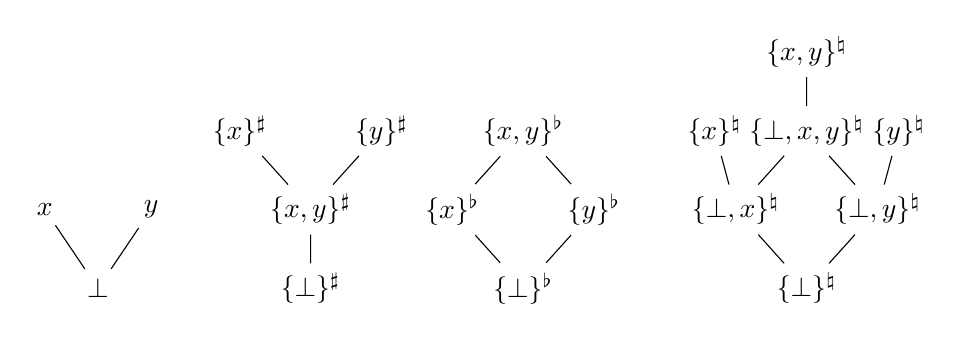
\begin{tikzpicture}[xscale=0.9]
  \node (U) at (0,0) {$\bot$};
  \node (A) at (-0.75,1) {$x$};
  \node (B) at (0.75,1) {$y$};
  \draw (A) -- (U) -- (B);
  
  \node (U1) at (3,0) {$\{\bot\}^\sharp$};
  \node (AB1) at (3,1) {$\{x,y\}^\sharp$};
  \node (A1) at (2,2) {$\{x\}^\sharp$};
  \node (B1) at (4,2) {$\{y\}^\sharp$};
  \draw (U1) -- (AB1);
  \draw (A1) -- (AB1) -- (B1);
  
  \node (U2) at (6,0) {$\{\bot\}^\flat$};
  \node (UA2) at (5,1) {$\{x\}^\flat$};
  \node (UAB2) at (6,2) {$\{x,y\}^\flat$};
  \node (UB2) at (7,1) {$\{y\}^\flat$};
  \draw (U2) -- (UA2) -- (UAB2);
  \draw (U2) -- (UB2) -- (UAB2);

  \node (U3) at (10,0) {$\{\bot\}^\natural$};
  \node (UA3) at (9,1) {$\{\bot,x\}^\natural$};
  \node (UB3) at (11,1) {$\{\bot,y\}^\natural$};
  \node (UAB3) at (10,2) {$\{\bot,x,y\}^\natural$};
  \node (A3) at (8.7,2) {$\{x\}^\natural$};
  \node (B3) at (11.3,2) {$\{y\}^\natural$};
  \node (AB3) at (10,3) {$\{x,y\}^\natural$};
  \draw (U3) -- (UA3) -- (A3);
  \draw (U3) -- (UB3) -- (B3);
  \draw (UA3) -- (UAB3);
  \draw (UB3) -- (UAB3);
  \draw (UAB3) -- (AB3);
\end{tikzpicture}
\par\end{centering}

\caption{\label{fig:lifted2}Lifted two-element type, with upper, lower, and
convex powerdomains}

\end{figure}


%
\begin{figure}
\begin{centering}
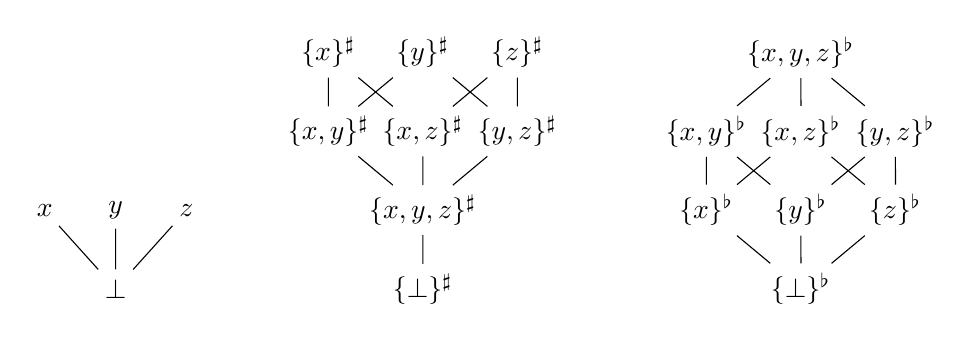
\begin{tikzpicture}[xscale=1.2]
  \node (U) at (0.75,0) {$\bot$};
  \node (A) at (0,1) {$x$};
  \node (B) at (0.75,1) {$y$};
  \node (C) at (1.5,1) {$z$};
  \draw (U) -- (A);
  \draw (U) -- (B);
  \draw (U) -- (C);

  \node (U1) at (4,0) {$\{\bot\}^\sharp$};
  \node (ABC1) at (4,1) {$\{x,y,z\}^\sharp$};
  \node (AB1) at (3,2) {$\{x,y\}^\sharp$};
  \node (BC1) at (5,2) {$\{y,z\}^\sharp$};
  \node (CA1) at (4,2) {$\{x,z\}^\sharp$};
  \node (A1) at (3,3) {$\{x\}^\sharp$};
  \node (B1) at (4,3) {$\{y\}^\sharp$};
  \node (C1) at (5,3) {$\{z\}^\sharp$};
  \draw (U1) -- (ABC1);
  \draw (ABC1) -- (AB1) -- (A1) -- (CA1);
  \draw (ABC1) -- (BC1) -- (B1) -- (AB1);
  \draw (ABC1) -- (CA1) -- (C1) -- (BC1);

  \node (U2) at (8,0) {$\{\bot\}^\flat$};
  \node (UA2) at (7,1) {$\{x\}^\flat$};
  \node (UB2) at (8,1) {$\{y\}^\flat$};
  \node (UC2) at (9,1) {$\{z\}^\flat$};
  \node (UAB2) at (7,2) {$\{x,y\}^\flat$};
  \node (UBC2) at (9,2) {$\{y,z\}^\flat$};
  \node (UCA2) at (8,2) {$\{x,z\}^\flat$};
  \node (UABC2) at (8,3) {$\{x,y,z\}^\flat$};
  \draw (U2) -- (UA2) -- (UAB2);
  \draw (U2) -- (UB2) -- (UBC2);
  \draw (U2) -- (UC2) -- (UCA2);
  \draw (UA2) -- (UCA2) -- (UABC2);
  \draw (UB2) -- (UAB2) -- (UABC2);
  \draw (UC2) -- (UBC2) -- (UABC2);
\end{tikzpicture}
\par\end{centering}

\caption{\label{fig:lifted3}Lifted three-element type, with upper and lower
powerdomains}

\end{figure}


%
\begin{figure}
\begin{centering}
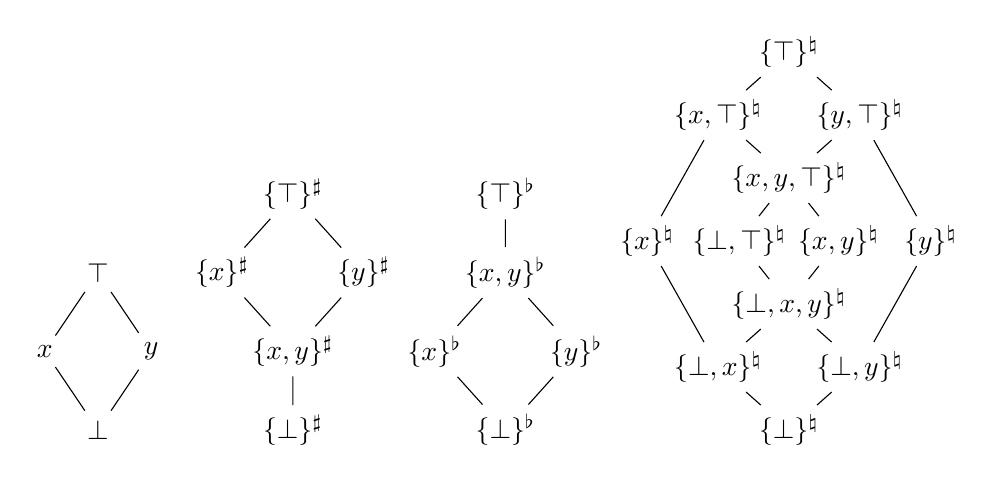
\begin{tikzpicture}[xscale=0.9]
  \node (U) at (1.25,0) {$\bot$};
  \node (A) at (0.5,1) {$x$};
  \node (B) at (2,1) {$y$};
  \node (T) at (1.25,2) {$\top$};
  \draw (U) -- (A) -- (T) -- (B) -- (U);
  
  \node (U1) at (4,0) {$\{\bot\}^\sharp$};
  \node (AB1) at (4,1) {$\{x,y\}^\sharp$};
  \node (A1) at (3,2) {$\{x\}^\sharp$};
  \node (B1) at (5,2) {$\{y\}^\sharp$};
  \node (T1) at (4,3) {$\{\top\}^\sharp$};
  \draw (U1) -- (AB1) -- (A1) -- (T1) -- (B1) -- (AB1);

  \node (U2) at (7,0) {$\{\bot\}^\flat$};
  \node (A2) at (6,1) {$\{x\}^\flat$};
  \node (B2) at (8,1) {$\{y\}^\flat$};
  \node (AB2) at (7,2) {$\{x,y\}^\flat$};
  \node (T2) at (7,3) {$\{\top\}^\flat$};
  \draw (T2) -- (AB2) -- (B2) -- (U2) -- (A2) -- (AB2);
  
  \node (U3) at (11,0) {$\{\bot\}^\natural$};
  \node (UA3) at (10,0.8) {$\{\bot,x\}^\natural$};
  \node (UB3) at (12,0.8) {$\{\bot,y\}^\natural$};
  \node (UAB3) at (11,1.6) {$\{\bot,x,y\}^\natural$};
  \node (A3) at (9,2.4) {$\{x\}^\natural$};
  \node (B3) at (13,2.4) {$\{y\}^\natural$};
  \node (UT3) at (10.3,2.4) {$\{\bot,\top\}^\natural$};
  \node (AB3) at (11.7,2.4) {$\{x,y\}^\natural$};
  \node (ABT3) at (11,3.2) {$\{x,y,\top\}^\natural$};
  \node (AT3) at (10,4.0) {$\{x,\top\}^\natural$};
  \node (BT3) at (12,4.0) {$\{y,\top\}^\natural$};
  \node (T3) at (11,4.8) {$\{\top\}^\natural$};
  \draw (U3) -- (UA3) -- (UAB3);
  \draw (U3) -- (UB3) -- (UAB3);
  \draw (UA3) -- (A3) -- (AT3);
  \draw (UB3) -- (B3) -- (BT3);
  \draw (UAB3) -- (UT3) -- (ABT3);
  \draw (UAB3) -- (AB3) -- (ABT3);
  \draw (ABT3) -- (AT3) -- (T3);
  \draw (ABT3) -- (BT3) -- (T3);

\end{tikzpicture}
\par\end{centering}

\caption{\label{fig:lattice4}Four-element lattice, with upper, lower, and
convex powerdomains}

\end{figure}



\section{\label{sec:HOLCF-powerdomain-library}HOLCF powerdomain library}

This section describes the user-visible aspects of the HOLCF powerdomain
library. The implementation defines three new type constructors, one
for each of the three powerdomain varieties. Each type has \texttt{unit}
and \texttt{plus} constructors, and a monadic \texttt{bind} operator.
Each type also has \texttt{map} and \texttt{join} operators, defined
in terms of \texttt{unit} and \texttt{bind} in the same manner as
Haskell's \texttt{liftM} and \texttt{join}. The full list of types
and constants is shown in Fig. \ref{fig:type-signatures}.

The functions \texttt{convex\_to\_lower} and \texttt{convex\_to\_upper}
are the mappings guaranteed to exist by the universal property of
the convex powerdomain; they preserve \texttt{unit} and \texttt{plus}.
Note that instead of the full function space (\texttt{=>}), all functions
use the HOLCF continuous function space type (\texttt{->}), indicating
that they are continuous functions.

%
\begin{figure}
\begin{verbatim}
typedef 'a upper_pd
upper_unit :: 'a -> 'a upper_pd
upper_plus :: 'a upper_pd -> 'a upper_pd -> 'a upper_pd
upper_bind :: 'a upper_pd -> ('a -> 'b upper_pd) -> 'b upper_pd
upper_map :: ('a -> 'b) -> 'a upper_pd -> 'b upper_pd
upper_join :: 'a upper_pd upper_pd -> 'a upper_pd

typedef 'a lower_pd
lower_unit :: 'a -> 'a lower_pd
lower_plus :: 'a lower_pd -> 'a lower_pd -> 'a lower_pd
lower_bind :: 'a lower_pd -> ('a -> 'b lower_pd) -> 'b lower_pd
lower_map :: ('a -> 'b) -> 'a lower_pd -> 'b lower_pd
lower_join :: 'a lower_pd lower_pd -> 'a lower_pd

typedef 'a convex_pd
convex_unit :: 'a -> 'a convex_pd
convex_plus :: 'a convex_pd -> 'a convex_pd -> 'a convex_pd
convex_bind :: 'a convex_pd -> ('a -> 'b convex_pd) -> 'b convex_pd
convex_map :: ('a -> 'b) -> 'a convex_pd -> 'b convex_pd
convex_join :: 'a convex_pd convex_pd -> 'a convex_pd
convex_to_upper :: 'a convex_pd -> 'a upper_pd
convex_to_lower :: 'a convex_pd -> 'a lower_pd
\end{verbatim}

\caption{\label{fig:type-signatures}Powerdomain types and constants defined
in HOLCF}

\end{figure}


For convenience, the library also provides set-style syntax for \texttt{unit}
and \texttt{plus}, similar to the notation used in this paper.

Along with the definitions of types and constants, the library provides
a significant body of lemmas. Each powerdomain type has an induction
rule in terms of \texttt{unit} and \texttt{plus}. Rules about injectivity,
strictness, compactness, and ordering are provided for the constructors.
Also, the functor and monad laws are provided as lemmas.


\subsection{Bifinite type class}

HOLCF uses Isabelle's axiomatic type class mechanism \cite{wenzel97typeclass}
to represent different kinds of domains. The main axiomatic type classes
in HOLCF are \texttt{cpo} (chain-complete partial orders) and \texttt{pcpo}
(pointed cpos). Unfortunately, the powerdomain constructions do not
work over arbitrary cpos; they need some additional structure. In
order to formalize powerdomains in HOLCF, it was necessary to add
a new axiomatic class \texttt{bifinite}, which is a subclass of \texttt{pcpo}.
I will have more to say about class \texttt{bifinite} in Section \ref{sec:Implementation}.

As far as a user of the library is concerned, it does not matter how
class \texttt{bifinite} is defined; the important thing is that it
should be preserved by all of type constructors that the user works
with. In the current version of Isabelle, instances are provided for
all type constructors defined in the HOLCF library: continuous function
space, Cartesian product, strict product, strict sum, lifted cpos,
and all three varieties of powerdomains. Flat domains built from countable
HOL types are instances of \texttt{bifinite} as well.

A known problem is that the current implementation of the domain package
does not generate instances of class \texttt{bifinite} for new types.
In the current version of HOLCF, if a user wants to use a domain package--defined
type with powerdomains, it will be necessary to manually prove that
the type is an instance of class \texttt{bifinite}. Updating the domain
package to work with the \texttt{bifinite} class is planned as future
work.


\subsection{Automation}

To facilitate reasoning with powerdomains, the library provides various
sets of rewrite rules that are designed to work well together.


\subsubsection{ACI normalization.}

Isabelle's simplifier is set up to handle permutative rewrite rules.
For any associative-commutative operator, there is a set of three
permutative rewrite rules that can convert any expression built from
the operator into a normal form (grouped to the right, with terms
sorted according to some term-ordering).\cite{baader1998} Two of
the AC rewrites are simply the associativity and commutativity rules.
The third is the left-commutativity rule. For ACI rewriting, we need
a total of five rules: the three AC rewrites, plus the idempotency
rule, and also (analogous to left-commutativity) left-idempotency.\begin{eqnarray}
(xs\cup ys)\cup zs & = & xs\cup(ys\cup zs)\nonumber \\
ys\cup xs & = & xs\cup ys\nonumber \\
ys\cup(xs\cup zs) & = & xs\cup(ys\cup zs)\label{eq:plus-aci}\\
xs\cup xs & = & xs\nonumber \\
xs\cup(xs\cup ys) & = & xs\cup ys\nonumber \end{eqnarray}


Permutative rewriting using the ACI rules results in a normal form
where expressions are nested to the right, and the terms are in sorted
order, with no exact duplicates. In HOLCF, this normalization can
be accomplished for the convex powerdomains by invoking \texttt{(simp
add: convex\_plus\_aci)}. Similarly, \texttt{upper\_plus\_aci} and
\texttt{lower\_plus\_aci} may be used with upper and lower powerdomains,
respectively.


\subsubsection{Solving inequalities.}

A common subgoal in a proof might be to show that one powerdomain
expression approximates another. For each variety of powerdomain,
there is a set of rewrites that can be used to automatically reduce
an inequality on powerdomains down to inequalities on the underlying
type.\begin{eqnarray}
\{x\}^{\sharp}\sqsubseteq\{y\}^{\sharp} & \iff & x\sqsubseteq y\nonumber \\
xs\sqsubseteq(ys\cup^{\sharp}zs) & \iff & (xs\sqsubseteq ys)\wedge(xs\sqsubseteq zs)\label{eq:upper-less}\\
(xs\cup^{\sharp}ys)\sqsubseteq\{z\}^{\sharp} & \iff & (xs\sqsubseteq\{z\}^{\sharp})\vee(ys\sqsubseteq\{z\}^{\sharp})\nonumber \end{eqnarray}
\begin{eqnarray}
\{x\}^{\flat}\sqsubseteq\{y\}^{\flat} & \iff & x\sqsubseteq y\nonumber \\
(xs\cup^{\flat}ys)\sqsubseteq zs & \iff & (xs\sqsubseteq zs)\wedge(ys\sqsubseteq zs)\label{eq:lower-less}\\
\{x\}^{\flat}\sqsubseteq(ys\cup^{\flat}zs) & \iff & (\{x\}^{\flat}\sqsubseteq ys)\vee(\{x\}^{\flat}\sqsubseteq zs)\nonumber \end{eqnarray}
\begin{eqnarray}
\{x\}^{\natural}\sqsubseteq\{y\}^{\natural} & \iff & x\sqsubseteq y\nonumber \\
\{x\}^{\natural}\sqsubseteq(ys\cup^{\natural}zs) & \iff & (\{x\}^{\natural}\sqsubseteq ys)\wedge(\{x\}^{\natural}\sqsubseteq zs)\label{eq:convex-less}\\
(xs\cup^{\natural}ys)\sqsubseteq\{z\}^{\natural} & \iff & (xs\sqsubseteq\{z\}^{\natural})\wedge(ys\sqsubseteq\{z\}^{\natural})\nonumber \end{eqnarray}


For the upper and lower powerdomains, each has a set of three rewrite
rules that covers all cases of comparisons. For example, invoking
\texttt{(simp add: upper\_pd\_less\_simps)} will rewrite $\{x,y\}^{\sharp}\sqsubseteq\{y,z\}^{\sharp}$
to $x\sqsubseteq z\vee y\sqsubseteq z$, using the rules in Eq. (\ref{eq:upper-less}).
Similarly, \texttt{(simp add: lower\_pd\_less\_simps)} uses the rules
in Eq. (\ref{eq:lower-less}) to simplify inequalities on lower powerdomains.

For the convex powerdomain, the three rules in Eq. (\ref{eq:convex-less})
are incomplete: They do not cover the case of $(xs\cup^{\natural}ys)\sqsubseteq(zs\cup^{\natural}ws)$.
To handle this case, we will take advantage of the coercions from
the convex powerdomain to the upper and lower powerdomains, along
with the following ordering property:\begin{eqnarray}
xs\sqsubseteq ys & \Longleftrightarrow & \mbox{to\_upper}(xs)\sqsubseteq\mbox{to\_upper}(ys)\wedge\mbox{to\_lower}(xs)\sqsubseteq\mbox{to\_lower}(ys)\label{eq:convex-less2}\end{eqnarray}
The rule set \texttt{convex\_pd\_less\_simps} includes all rules from
Eqs. (\ref{eq:upper-less})--(\ref{eq:convex-less}), and a suitably
instantiated Eq. (\ref{eq:convex-less2}) to cover the missing case.


\subsubsection{Using inequalities to solve non-trivial equalities.}

The ACI rewriting can take care of many equalities between powerdomain
expressions, but the inequality rules can actually solve more. For
example, using the assumptions $x\sqsubseteq y$ and $y\sqsubseteq z$,
we will prove that $\{x,y,z\}^{\natural}=\{x,z\}^{\natural}$. By
antisymmetry, we can rewrite this to the conjunction $(\{x,y,z\}^{\natural}\sqsubseteq\{x,z\}^{\natural})\wedge(\{x,z\}^{\natural}\sqsubseteq\{x,y,z\}^{\natural})$.
Next, we can use the method \texttt{(simp add: convex\_pd\_less\_simps)},
and this subgoal reduces to $(y\sqsubseteq x\vee y\sqsubseteq z)\wedge(x\sqsubseteq y\vee z\sqsubseteq y)$.
Finally, this is easily discharged using the assumptions $x\sqsubseteq y$
and $y\sqsubseteq z$.


\section{\label{sec:Implementation}Implementation}

The development of powerdomains in HOLCF follows the ideal completion
construction presented by Gunter and Scott in \cite[\S5.2]{gunter90semantic}.
Some alternative constructions are also given by Abramsky and Jung
in \cite[\S6.2]{abramsky94domain}; the ideal completion method was
chosen because it required the formalization of a minimal amount of
supporting theories, and it offered good opportunities for proof reuse.


\subsection{Class of bifinite domains}

The powerdomain construction used in HOLCF makes use of an alternative
representation of domains, where we just consider the set of compact
(i.e. finite) values, rather than the whole domain.\cite[\S2.2.6]{abramsky94domain}
For this representation to work, we restrict our attention to \emph{algebraic}
cpos, where every value can be expressed as the limit of its compact
approximants. This means that in an algebraic cpo the set of compact
elements, together with the domain ordering on them, fully represents
the entire domain. We say that the set of compact elements forms a
\emph{basis} for the domain, and the entire domain is a \emph{completion}
of the basis.

Most of HOLCF has been designed using the type class \texttt{pcpo}
of pointed complete partial orders. However, \texttt{pcpo} types are
not algebraic in general, and the ideal completion construction only
works with algebraic cpos. Therefore it was necessary to add a new
type class to HOLCF.

The class \texttt{bifinite} is defined as follows. It fixes a sequence
of functions $\mbox{approx}_{n}$, and assumes four class axioms:

\begin{enumerate}
\item The $\mbox{approx}_{n}$ form a chain
\item The least upper bound $(\bigsqcup_{n}\mbox{approx}_{n})$ is the identity
function
\item Each $\mbox{approx}_{n}$ is idempotent
\item Each $\mbox{approx}_{n}$ has finite range
\end{enumerate}
The HOLCF \texttt{bifinite} class actually corresponds to the {}``$\omega$-bifinite''
domains, which have a countable basis; the usual definition of {}``bifinite''
\cite[\S4.2]{abramsky94domain} has no such restriction, and would
be equivalent to allowing any directed set of approx functions, rather
than a countable chain. Bifinite domains were originally defined by
Plotkin as limits of expanding sequences of finite posets, who used
the name {}``SFP domain''.\cite{plotkin76powerdomain}

Of all the various classes of domains to choose from, the definition
of \texttt{bifinite} was chosen for the following reasons:

\begin{itemize}
\item All \texttt{bifinite} types are algebraic: Every \texttt{bifinite}
type has a countable basis of compact elements, given by the union
of the ranges of the approx functions.
\item In \texttt{bifinite} types, every directed set contains a chain with
the same limit. This means that in class \texttt{bifinite}, the notions
of directed-continuity and chain-continuity coincide. This is important
for fitting the ideal completion construction (which uses directed
sets) into HOLCF (which defines everything with chains).
\item The \texttt{bifinite} class is closed under all type constructors
used in HOLCF, including the convex powerdomain.
\end{itemize}

\subsection{Ideal completion}

Given a basis $\left\langle B,\preceq\right\rangle $, we can reconstruct
the full algebraic cpo. The standard process for doing this is called
ideal completion, and it is done by considering the set of ideals
over the basis:

\begin{definition}
A set $S$ is an \emph{ideal} with respect to partial preorder relation
$(\preceq)$ if it has the following properties:
\begin{itemize}
\item $S$ is nonempty: $\exists x.\, x\in S$
\item $S$ is downward-closed: $\forall x\, y.\, x\preceq y\longrightarrow y\in S\longrightarrow x\in S$
\item $S$ is directed (i.e. has an upper bound for any pair of elements):\\
 $\forall x\, y.\, x\in S\longrightarrow y\in S\longrightarrow(\exists z.\, z\in S\wedge x\preceq z\wedge y\preceq z)$
\end{itemize}
A \emph{principal} \emph{ideal} is an ideal of the form $\{y.\, y\preceq x\}$
for some $x$, denoted $\downarrow\! x$.
\end{definition}
The set of all ideals over $\left\langle B,\preceq\right\rangle $
is denoted $\mbox{Idl}(B)$; when ordered by subset inclusion, $\mbox{Idl}(B)$
forms an algebraic cpo. The compact elements of $\mbox{Idl}(B)$ are
exactly those represented by principal ideals.

Note that the relation $(\preceq)$ does not need to be antisymmetric.
For $x$ and $y$ that are equivalent (that is, both $x\preceq y$
and $y\preceq x$) the principal ideals $\downarrow\! x$ and $\downarrow\! y$
are equal. This means that the ideal completion construction automatically
takes care of quotienting by the equivalence induced by $(\preceq)$.

The ideal completion construction is formalized in HOLCF using Isabelle's
locale mechanism.\cite{kammuller99locales} The library defines a
locale \texttt{preorder} that fixes a type corresponding to the basis
$B$, and a preorder relation on that type; within this locale, a
predicate \texttt{ideal} is defined. Within the \texttt{preorder}
locale, the main lemma proved is that the union of a chain of ideals
is itself an ideal---which shows that the ideal completion is a cpo.

All three of the powerdomains in the library are defined by ideal
completion. For an basis, the library defines a type \texttt{'a pd\_basis},
which consists of nonempty, finite sets of compact elements of type
\texttt{'a}. Following \cite[\S5.2]{gunter90semantic}, each of the
three powerdomains is defined as an ideal completion over the same
basis, but each uses a different preorder relation:\begin{eqnarray}
a\preceq^{\flat}b & \iff & \forall x\in a.\ \exists y\in b.\ x\sqsubseteq y\nonumber \\
a\preceq^{\sharp}b & \iff & \forall y\in b.\ \exists x\in a.\ x\sqsubseteq y\label{eq:preorders}\\
a\preceq^{\natural}b & \iff & a\preceq^{\flat}b\wedge a\preceq^{\sharp}b\nonumber \end{eqnarray}



\subsection{Continuous extensions of functions}

A continuous function on an algebraic cpo is completely determined
by its action on compact elements. This suggests a method for defining
continuous functions over ideal completions: First, define a function
from the basis $B$ to a cpo $C$ such that $f$ is monotone, i.e.
$x\preceq y$ implies $f(x)\sqsubseteq f(y)$. Then there exists a
unique function $\hat{f}:\mbox{Idl}(B)\rightarrow C$ that agrees
with $f$ on principal ideals, i.e. for all $x$, $\hat{f}(\downarrow\! x)=f(x)$.
We say that $\widehat{f}$ is the \emph{continuous extension} of $f$.

On top of the \texttt{preorder} locale, HOLCF defines another locale
\texttt{ideal\_completion} which fixes a second type corresponding
to $\mbox{Idl}(B)$. It also fixes a function \texttt{principal} of
type $B\rightarrow\mbox{Idl}(B)$. Within this locale, a function
\texttt{basis\_fun} is defined, which takes a monotone function $f$
as an argument, and returns the continuous extension $\widehat{f}$.

The continuous extension is defined by mapping the function $f$ over
the input ideal, and then taking the least upper bound of the resulting
directed set: $\widehat{f}(S)=\bigsqcup_{x\in S}f(x)$. Ordinarily,
the result type $C$ would need to be a directed-complete partial
order to ensure that this least upper bound exists; however, the HOLCF
library uses a different method which allows $C$ to be any chain-complete
partial order.

HOLCF defines a third locale \texttt{basis\_take}, which fixes a chain
of \texttt{take} functions over the basis elements---it is like a
version of the \texttt{bifinite} class for bases. The \texttt{basis\_take}
locale ensures that the ideal completion $\mbox{Idl}(B)$ is a bifinite
domain. It is also used with the definition of \texttt{basis\_fun}
to construct a chain with the same limit as the directed set $\bigsqcup_{x\in S}f(x)$,
which allows $C$ to be an arbitrary chain-cpo.

The \texttt{basis\_fun} combinator is used to define the powerdomain
constructors \texttt{unit} and \texttt{plus} in terms of the singleton
and union operations on the \texttt{pd\_basis} type. The \texttt{bind}
operators are also defined using \texttt{basis\_fun}, in terms of
a finite-set fold operation on \texttt{pd\_basis}. Finally, to prove
the \texttt{bifinite} class instance, the approx functions are also
defined with \texttt{basis\_fun}, in terms of the \texttt{take} functions
on \texttt{pd\_basis}.


\subsection{Transferring properties to the completed domain}

Once the powerdomain types are defined using ideal completion, with
operations defined by continuous extension, the final step is to prove
the relevant lemmas. For example, consider the lower powerdomain law
$xs\sqsubseteq xs\cup^{\flat}ys$. In the case where $xs$ and $ys$
are both compact (i.e. represented by principal ideals) the proof
follows easily from the definitions. Since $xs\sqsubseteq xs\cup^{\flat}ys$
is an admissible predicate on both $xs$ and $ys$, this is in fact
sufficient to show that it holds for all $xs$ and $ys$.

Other properties are more tricky to transfer. For example, consider
the rule $\{x\}^{\natural}\sqsubseteq\{y\}^{\natural}\Longrightarrow x\sqsubseteq y$.
As before, this property is easy to prove for compact $x$ and $y$.
However, we cannot immediately infer that it holds for all $x$ and
$y$, since (because of the implication) this is not an admissible
predicate.

The proof of $\{x\}^{\natural}\sqsubseteq\{y\}^{\natural}\Longrightarrow x\sqsubseteq y$
requires a few extra steps, making use of the approx functions from
the \texttt{bifinite} class: To prove $x\sqsubseteq y$, it will be
sufficient to show that for all $n$, $\mbox{approx}_{n}x\sqsubseteq\mbox{approx}_{n}y$.
Now, from $\{x\}^{\natural}\sqsubseteq\{y\}^{\natural}$ we have $\mbox{approx}_{n}\{x\}^{\natural}\sqsubseteq\mbox{approx}_{n}\{y\}^{\natural}$,
by monotonicity; then from the definition of approx on the convex
powerdomain, this simplifies to $\{\mbox{approx}_{n}x\}^{\natural}\sqsubseteq\{\mbox{approx}_{n}y\}^{\natural}$.
Finally, since $\mbox{approx}_{n}x$ and $\mbox{approx}_{n}y$ are
compact, we can easily show that $\mbox{approx}_{n}x\sqsubseteq\mbox{approx}_{n}y$.
All of the rules listed in Eqs. (\ref{eq:upper-less})--(\ref{eq:convex-less2})
use a similar proof.


\section{Related work}

There are several theorem prover formalizations of domain theory in
existence. The current development is built on top of HOLCF, originally
implemented by Regensburger, and later extended by many others.\cite{regensburger95holcf,MuellerNvOS99}
HOLCF does not formalize very many different classes of domains; most
concepts are defined in terms of pointed chain-complete partial orders
and chain-continuity, which is the minimum amount of structure required
to define a fixed-point combinator. It is intended to be used as a
library for users to define datatypes and recursive functions and
algorithms on them.

In the mid-1990s a group from the University of Ulm formalized parts
of domain theory in PVS.\cite{BDvH+96} Its design goals appear to
be similar to HOLCF---it includes just enough of domain theory to
formalize fixed-points and fixed-point induction.

A formalization of domain theory with rather different goals is {}``Elements
of Domain Theory'', implemented in Coq in the 1990s by Kahn. It is
based on the definitions and lemmas from \cite{kahn93concretedomains}.
This development defines several classes of domains, including directed-complete
partial orders, omega-algebraic cpos, and bounded-complete domains.
However, it does not define any type constructors. In contrast to
HOLCF, it does not appear to be application-oriented; it seems the
main intent was to formalize the textbook-style definitions and lemmas
from the paper.

Other formalizations use a different logic to ensure that all functions
are continuous by construction, such as the LCF system by Paulson.\cite{paulson87lcf}
Another interesting approach is taken by Reus with his development
of synthetic domain theory in LEGO.\cite{reus96synthetic} Instead
of defining classes of domains in terms of a domain ordering, it starts
by introducing a \emph{subobject} \emph{classifier}, which is characterized
by a collection of axioms. The soundness of the construction is justified
by a separate model.

Relevant uses of powerdomains include modeling interleaved and parallel
computation. Papaspyrou uses the convex powerdomain, together with
the state and resumption monad transformers, to model impure languages
with unspecified evaluation order.\cite{papaspyrou00study} Along
similar lines, Thiemann used a type of state monad built on top of
powerdomains to reason about concurrent computations.\cite{thiemann95towards}
The monad transformers used in these works, specifically the resumption
monad transformer, have been studied in HOLCF by Huffman, et al.\cite{huffman05axiomatic}


\section{Conclusion and future work}

The powerdomain library described here is included as part of Isabelle2008
theorem prover. It can already be used to prove properties of simple
nondeterministic algorithms, with automation for certain kinds of
subgoals. Future work will focus on better integration with the HOLCF
domain package: Bifinite class instances must be generated for all
new datatypes. Also, the domain package needs to be extended to allow
recursive type definitions involving powerdomains---this will enable
the use of powerdomains for modeling parallel computation and concurrency.



\bibliographystyle{plain}
\bibliography{tphols08}

\end{document}
